\let\negmedspace\undefined
\let\negthickspace\undefined
\documentclass[journal,12pt,twocolumn]{IEEEtran}
\usepackage{cite}
\usepackage{amsmath,amssymb,amsfonts,amsthm}
\usepackage{algorithmic}
\usepackage{graphicx}
\usepackage{textcomp}
\usepackage{xcolor}
\usepackage{txfonts}
\usepackage{listings}
\usepackage{enumitem}
\usepackage{mathtools}
\usepackage{gensymb}
\usepackage{comment}
\usepackage[breaklinks=true]{hyperref}
\usepackage{tkz-euclide}
\usepackage{listings}
\usepackage{gvv}
\def\inputGnumericTable{}
\usepackage[latin1]{inputenc}
\usepackage{color}
\usepackage{array}
\usepackage{longtable}
\usepackage{calc}
\usepackage{multirow}
\usepackage{hhline}
\usepackage{ifthen}
\usepackage{lscape}
\usepackage{circuitikz}

\newtheorem{theorem}{Theorem}[section]
\newtheorem{problem}{Problem}
\newtheorem{proposition}{Proposition}[section]
\newtheorem{lemma}{Lemma}[section]
\newtheorem{corollary}[theorem]{Corollary}
\newtheorem{example}{Example}[section]
\newtheorem{definition}[problem]{Definition}
\newcommand{\BEQA}{\begin{eqnarray}}
\newcommand{\EEQA}{\end{eqnarray}}
\newcommand{\define}{\stackrel{\triangle}{=}}
\theoremstyle{remark}
\newtheorem{rem}{Remark}
\begin{document}

\bibliographystyle{IEEEtran}
\vspace{3cm}

\title{Gate 2023- Instrumentation Engineering}
\author{EE23BTECH11037 - M Esha$^{*}$% <-this % stops a space
}
\maketitle
\newpage
\bigskip

\renewcommand{\thefigure}{\theenumi}
\renewcommand{\thetable}{\theenumi}

\vspace{3cm}
\textbf{Question 59:} 
The op amps in the circuit are ideal. The input signals are $V_{S1} = 3 + 0.10 \sin(300t), \text{V}$ and $V_{S2} = -2 + 0.11 \sin(300t)\, \text{V}$. The average value of the voltage $V_0$ is \underline{\hspace{1cm}} volts (rounded off to two decimal places).

\begin{figure}[ht]
\centering
\resizebox{0.55\columnwidth}{!}{\begin{circuitikz}

% Lines
\draw (-2.5,2.5) -- (0.5,2.5);
\draw (0.5,3) -- (0.5,1);
\draw (0.5,1.5) -- (0,1.5);
\draw (0,1.5) -- (0,0);
\draw (-2.5,-4) -- (0.5,-4);
\draw (0.5,-4.5) -- (0.5,-2.5);
\draw (0.5,-3) -- (0,-3);
\draw (0,-3) -- (0,-1.5);
\draw (0.5,3) -- (2,2);
\draw (0.5,1) -- (2,2);
\draw (2,2) -- (3.5,2);
\draw (3.5,2) -- (5.5,2);
\draw (3.5,2) -- (3.5,1.5);
\draw (0.5,-2.5) -- (2,-3.5);
\draw (0.5,-4.5) -- (2,-3.5);
\draw (2,-3.5) -- (3.5,-3.5);
\draw (3.5,-3.5) -- (3.5,-3);
\draw (3.5,-3.5) -- (5.5,-3.5);
\draw (5.5,-3.5) -- (5.5,-2.25);
\draw (5.5,2) -- (5.5,0.75);
\draw (5.5,-0.75) -- (6.5,-0.75);
\draw (0,0) -- (3.5,0);
\draw (0,-1.5) -- (3.5,-1.5);
\draw (6.5,-1.5) -- (6.5,-2.5);
\draw (6.25,-2.5) -- (6.75,-2.5);
\draw (6.3,-2.55) -- (6.7,-2.55);


% Resistors
\draw (3.5,1.5) to [resistor] (3.5,0);
\draw (3.5,0) to [resistor] (3.5,-1.5);
\draw (3.5,-1.5) to [resistor] (3.5,-3);
\draw (5.5,0.75) to [resistor] (5.5,-0.75);
\draw (5.5,-0.75) to [resistor] (5.5,-2.25);

% Labels
\node at (-3,2.5) {$V_{S1}$};
\node at (-3,-4) {$V_{S2}$};
\node at (0.75,2.5) {+};
\node at (0.75,1.5) {-};
\node at (0.75,-3) {-};
\node at (0.75,-4) {+};
\node at (7,-0.75) {$V_o$};
\node at (4.25,0.75) {R};
\node at (4.25,-0.75) {R};
\node at (4.25,-2.25) {R};
\node at (6.25,0) {R};
\node at (6.25,-1.5) {R};
\node at (6.75,-0.8) {+};
\node at (6.75,-1.5) {-};

% Dot 
\filldraw (6.5,-0.75) circle [radius=0.05];
\fill (6.5,-1.5) circle [radius=0.05]; 

\end{circuitikz}

}
\end{figure}
\hfill{(GATE IN 2023)}\\
\solution
\begin{table}[h!]
  \centering
  \begin{tabular}{|c|c|c|}
  \hline
  \textbf{Variable} & \textbf{Value} & \textbf{Description} \\
  \hline
  $V_{s1}$ & $3 + 0.10 \sin(300t)$ & \multirow{2}{*}{Input voltages} \\
  \cline{1-2}
  $V_{s2}$ & $-2 + 0.11 \sin(300t)$ & \\
  \cline{1-3}
  $R$ & & Resistances of the resistors \\
  \cline{1-3}
  $V_o$ & & Output voltage \\
  \cline{1-3}
  $V_1$ & & Output voltage of $V_{s1}$ opamp \\
  \cline{1-3}
  $V_2$ & & Output voltage of $V_{s2}$ opamp \\
  \hline
\end{tabular}

  \caption{Input Parameters}
    \label{tab:table1}
\end{table}\\
the current does not flow through op-amp. voltage drop by each R
\begin{align}
&= V_{s1}-V_{s2}
\end{align}
by KVL,
\begin{align}
V_{s2}-V_2&=V_{s1}-V_{s2}\\
V_2&=2V_{s2}-V_{s1}\\
V_1-V_{s1}&=V_{s1}-V_{s2}\\
V_1&= 2V_{s1}-V_{s2}\\
V_o&= \frac{V_1+V_2}{2}\\
&=\frac{V_{s1}+V_{s2}}{2}\\
&=\frac{3+0.10\sin(300t)+{-2}+0.11\sin(300t)}{2}\\
&=0.5+ \frac{0.21\sin(300t)}{2}\\
V_{avg}&=\frac{1}{T} \int_{0}^{T} V(t) \,dt\\
&=\frac{300}{2\pi} \int_{0}^{\frac{2\pi}{300}} \left(0.5 + \frac{0.21 \sin(300t)}{2}\right) \, dt\\
&=0.5
\end{align}
\begin{figure}[b]
    \centering
    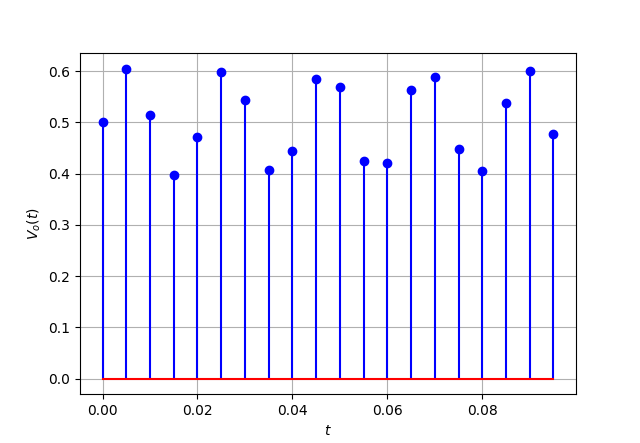
\includegraphics[width=\columnwidth]{59/figs/59fig.png}
    \caption{stem plot }
    \label{fig:1}
\end{figure}
\end{document}

